\section{Methodology}
\label{sec: Methodology}
% In this section. First, we describe the dataset. Second we show how we collecting data, preprocessing data for the model and the last we describe our algorithm.


A dataset is created using twitter (a popular micro-blogging service where users create status messages called tweets) posts of electronic products. These tweets sometimes express opinions about different topics. Therefore, they are short messages full of slang words and misspellings (Fig.\ref{fig1}).  So we propose a method to automatically classifying sentiment (positive or negative) from a tweet. This is done in three phases. In the first phase preprocessing is done. Then a feature vector is created using relevant features. Finally using SVM classifiers, tweets are classified into positive and negative classes. 

\begin{figure*}[!htb]
    \center{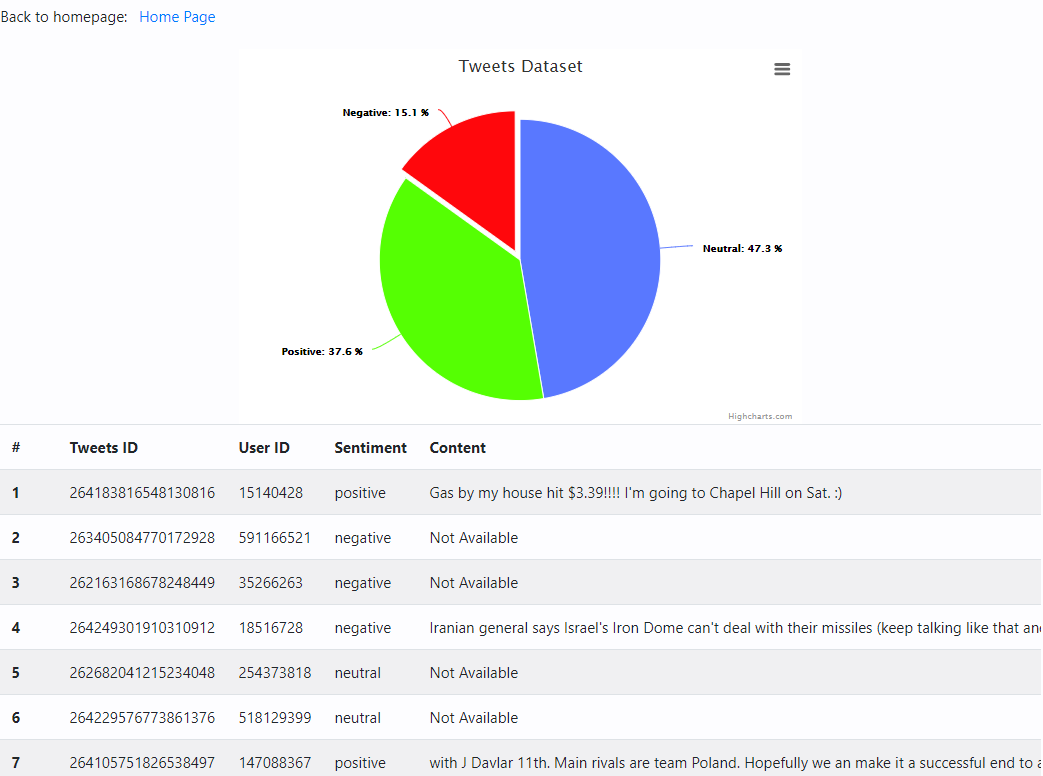
\includegraphics[width=1.4\columnwidth]{original_dataset.png}}
    \caption{\label{fig1} Original dataset}
\end{figure*}

\begin{figure*}[!htb]
    \center{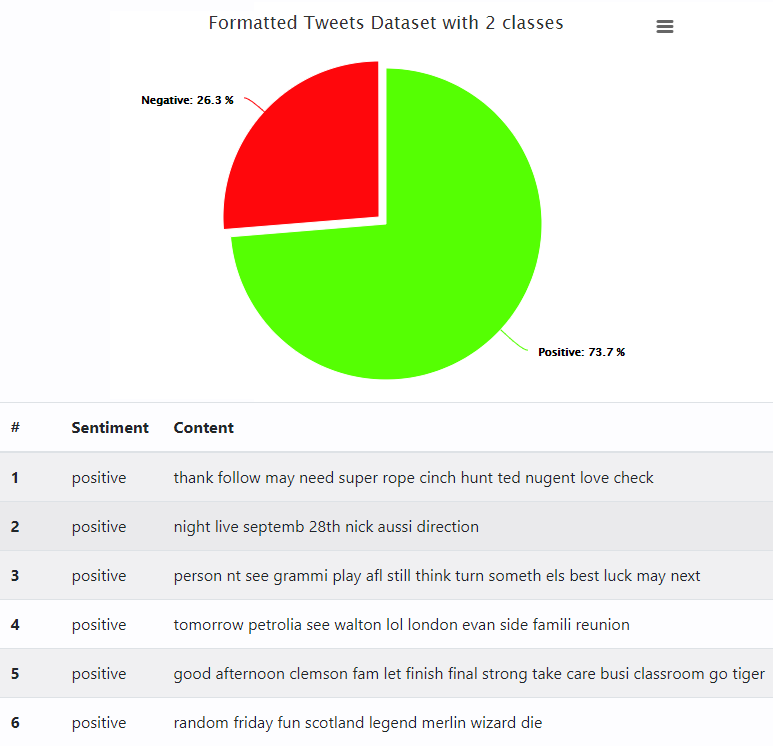
\includegraphics[width=1.4\columnwidth]{formatted_2classes.png}}
    \caption{\label{fig3} Our dataset after preprocessing}
\end{figure*}


\subsection{Dataset}
\label{sec: Dataset}

The data used in this project for training and testing is SemEval-2014 Twitter dataset Task 9 Corpus \cite{nakov2016evaluation} which was collected within the SemEval-2014 Task 9 competition that was a part of the International Workshop on Semantic Evaluation. We used 80$\%$ of the dataset for training and the remaining 20$\%$ for testing.


\subsection{Preprocessing Data}
\label{sec: Preprocessing Data}

A tweet contains a lot of opinions about the data which are expressed in different ways by different users. So keyword extraction is difficult on twitter due to misspellings and slang words. To avoid this, a preprocessing step is performed before feature extraction. Preprocessing steps include several techniques following to select features from the raw data: 

\begin{itemize}
    \item Remove all URLs (e.g. $www.xyz.com$), hash tags (e.g. $\#topic$), targets ($@$username), hyperlinks, numbers, repeated letters (more than 2 repeated letters) and punctuation marks.
    \item Removing stop words that add no sentiment value (articles, some prepositions, etc.).
    \item Stemming: reducing distinct words to their root form (stem).
    \item Removing infrequent words (words that appear less than $n_{min}$ number of times).
\end{itemize}

\subsection{Creation of Feature Vector}
\label{sec: Creation of Feature Vector}
 

\begin{figure}[!ht]
    \center{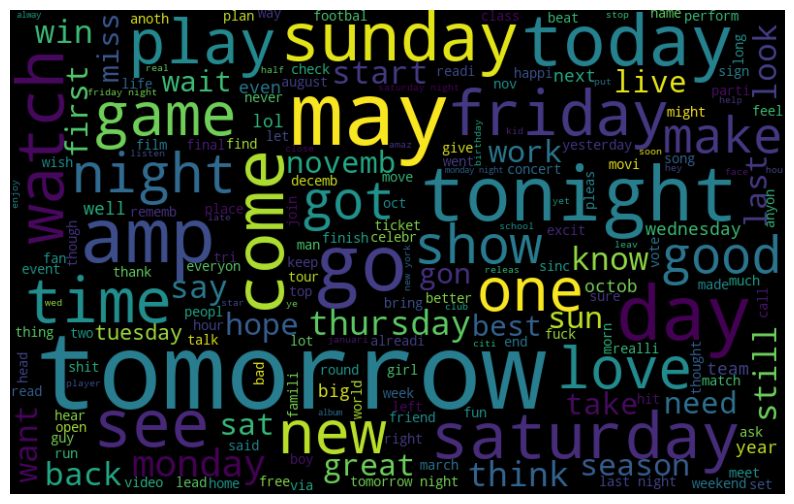
\includegraphics[width=1.0\columnwidth]{features.png}}
    \caption{\label{fig_feature_vector} Our features}
\end{figure}


For the unigram feature, there are usually a larger 500,000 different features. This is a very large number. It makes a model a higher variance. (Since the more complicated model has higher variance). It will need much more training data to avoid overfitting. Our dataset set contains almost 10 hundreds of sentences. This is a small number of examples. So we need to discard some useless features.

In this project, we use frequency-based feature selection which is the simplest way to do the feature selection. We just pick features (unigram words in our case) for each class with high-frequency occurrence in this class. In practice, if the number of occurrences of a feature is larger than some threshold (100 or 1000 in our experiments), this feature is a good one for that class (Fig.\ref{fig_feature_vector}). As we have seen in the result table, this simple algorithm increases about 0.03 of accuracy.



\subsection{Classification Technique}
\label{sec: Classification Technique}

There are different types of classifiers that are generally used for text classification which can be also used for twitter sentiment classification. But in this project, we focus on using  Support Vector Machine to do classify twitter sentiment.

SVM Classifier uses a large margin for classification. It separates the tweets using a hyperplane. SVM uses the discriminative function defined as

\begin{equation} \label{eq: svm}
g(X) = w^T \phi(X) + b
\end{equation}

$X$ is the feature vector, $w$ is the weights vector and $b$ is
the bias vector. $\phi()$ is the non-linear mapping from input space to high dimensional feature space. $w$ and $b$ are learned
automatically on the training set. Here we used different kernels for classification such as linear and radial basis functions. It maintains a wide gap between two classes.


\subsection{Automated Sentiment Classification System}
\label{sec: system}

After the training and testing process, we selected and saved the best model for later usage. After that, we built a web interface tool to aid in the manual user-defined query and then automated sentiment classification. 
 
After typing the user-query (query will be directly done by Twitter API).  The saved model is loaded and used to classify the tweets (return from twitter api). The statistics of the number of positive and negative tweets also are also calculated. The classification labels is compared between our model and TextBlob (\cite{loria2014textblob}) model (Fig.\ref{automated_system}).

\begin{figure*}[!t]
    \center{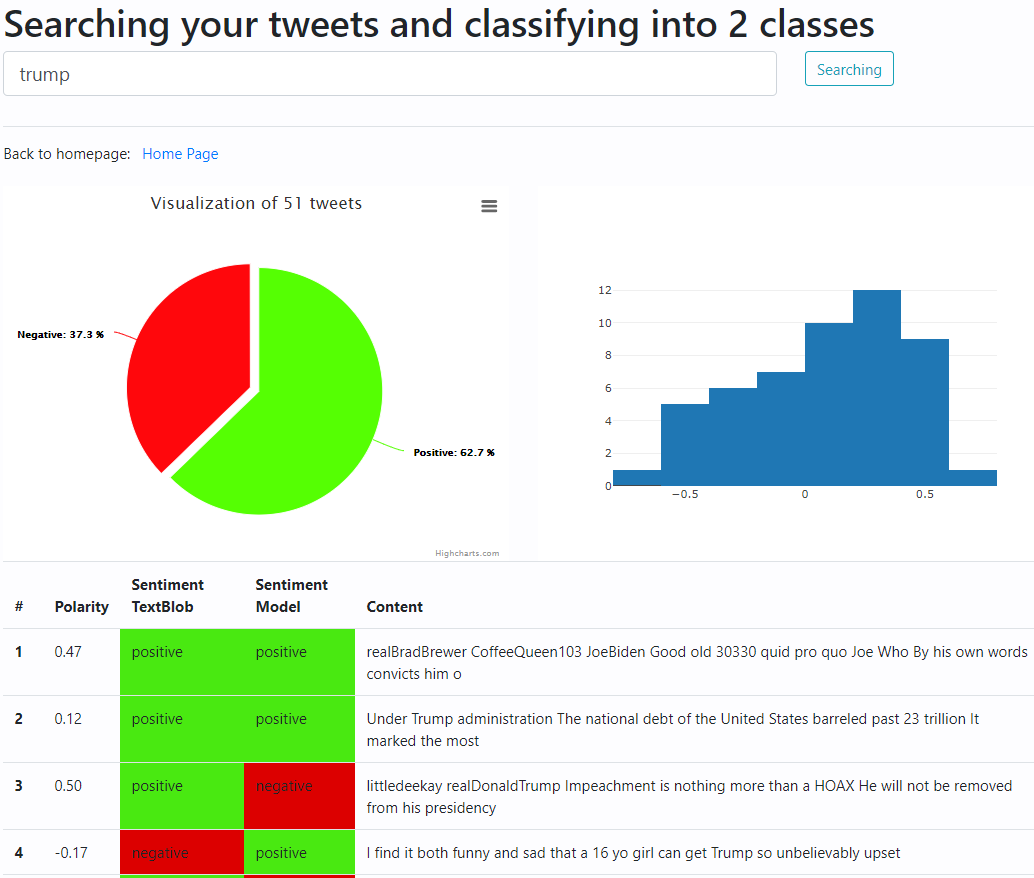
\includegraphics[width=1.8\columnwidth]{searching_and_comparing.png}}
    \caption{\label{automated_system} Automated sentiment classification system}
\end{figure*}


